\section{Schedule}
\label{ch:dp-tc-schedrisk}



\begin{dunefigure}[Overall installation schedule]{fig:overallSchedule}
{Overall installation schedule.}
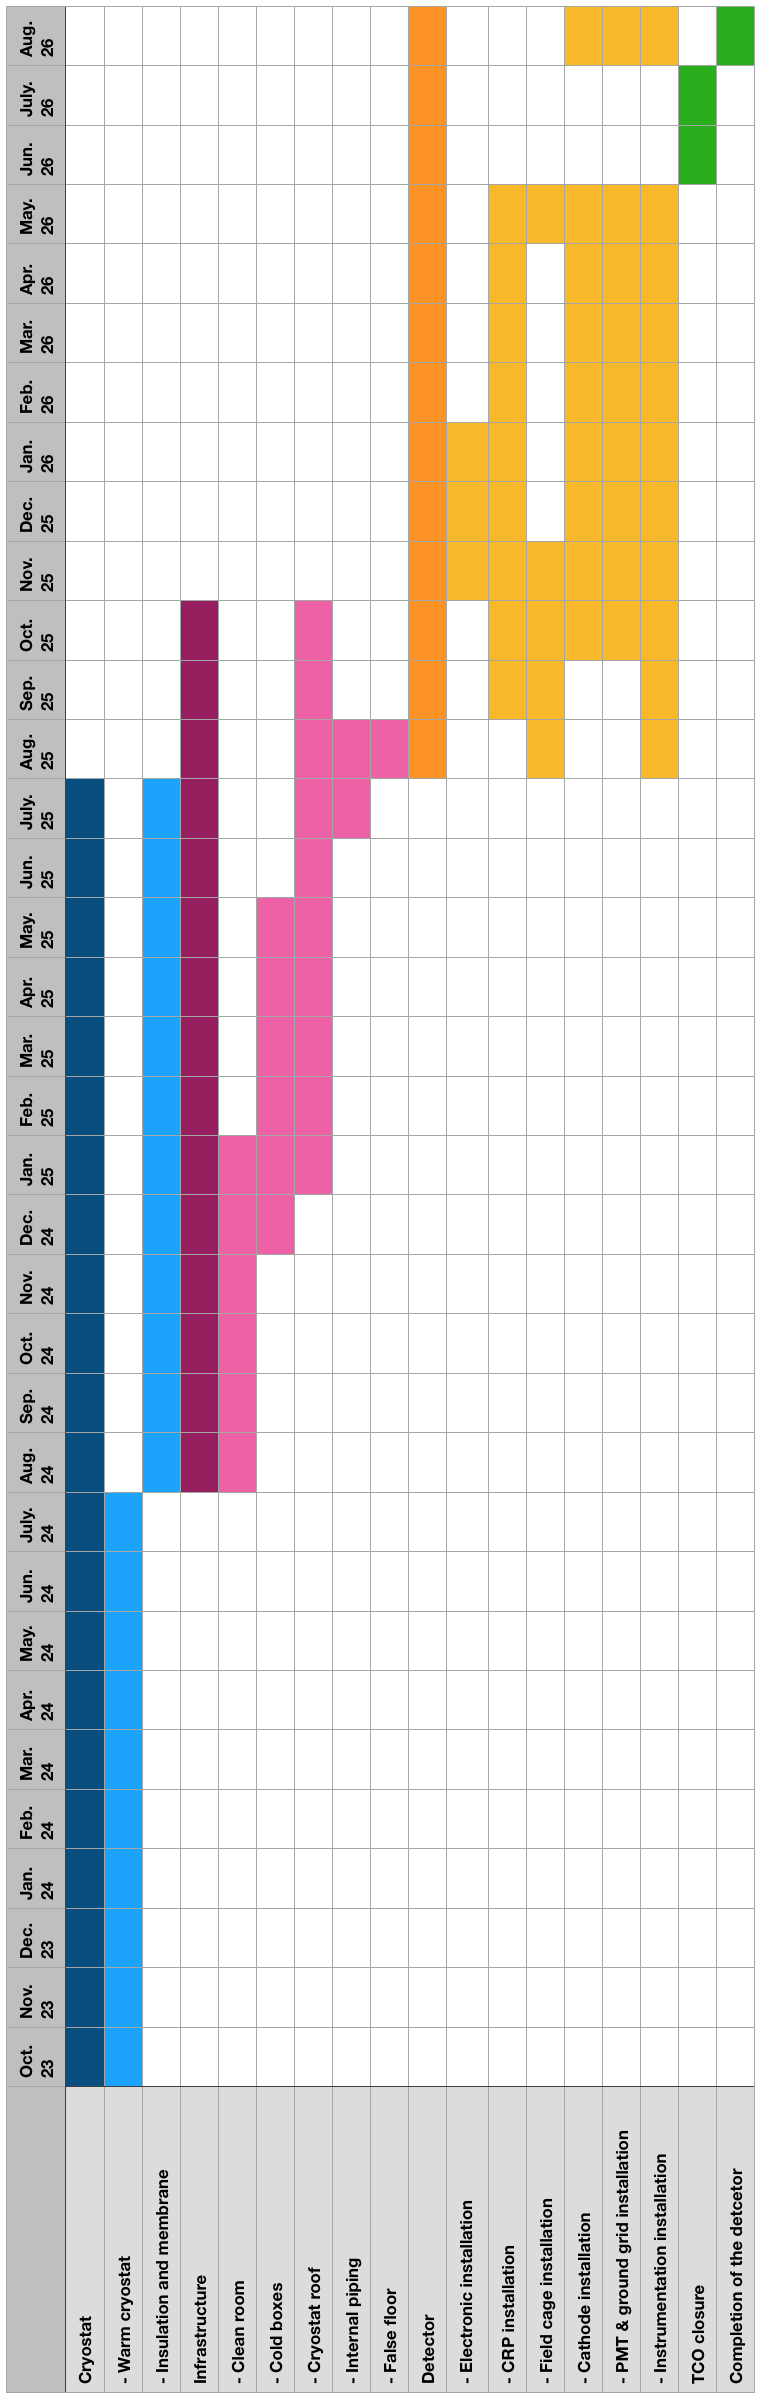
\includegraphics[width=0.4\textwidth]{overallSchedule.png}
\end{dunefigure}

Figure~\ref{fig:overallSchedule} show the overall schedule, (relative to a nominal start date that will be finalized following overall baselining of the LBNF project), from the beginning of the warm cryostat construction to the closure of the man-holes.
In this schedule, the construction of the warm part of the \dword{dp} cryostat will take ten months, and will be done in parallel to the installation of the cold part of the \dword{sp} cryostat.
The insulation and the primary containment system of the \dword{dp} cryostat will follow.
Twelve months are dedicated to this activity done in parallel with the \dword{sp} detector installation and with the \dword{dp} infrastructure installation.
At most 144 people are allowed to be underground at anytime.
Six months are allocated for the construction of the clean room, structure, walls, overhead crane, ventilation, power and lighting systems. 
The installation priority in this period is given to the insulation and membrane: the construction of the clean room should not interfere or slow down the cold part of the cryostat.
Before the completion of the clean room, the construction of the cold boxes and the related cryogenic system must begin.
The time allocated for this activity is six months and it is believed that given the co-activity in the clean room at this time, the allocated time is just right.
In the mean time, the installation of the infrastructure on the cryostat roof must commence.
Ten months are dedicated to the welding of all the support structure, the penetration pipes and flanges, installation of the racks, cable trays, purge pipes, walk-able floor, \dword{crp} and \dword{fc} supports and the \dwords{sgft}.
These last three items must be ready before the beginning of the \dword{tpc} installation.
The electronics instalation can start when the first \dwords{sgft} are available.
Once the cryostat is complete, internal cryogenic piping and the false floor will be installed before the actual detector installation will begin.
As explained in the previous section, the cryogenic instrumentation and the \dword{fc} will be the items installed first.
The installation of all the \dword{fc} except for the last end-wall will be done in four months.
After cryogenic tests in the cold box the \dwords{crp} will be installed at a constant pace for nine months.
The cathode, ground grid and \dword{pmt} installation will follow the advances in the \dword{crp} installation.
The \dword{fc} end-wall and the \dword{hv} extender will be installed just after the last \dword{crp} is installed, connected and tested.
The \dword{tco} closure activities are scheduled for two months and the last months is dedicated to the final cleaning or the detector and the cryostat.
Table~\ref{tab:milestones} summarizes the milestones for the \dword{dpmod} installation according to the global schedule just described.


\begin{dunetable}
[\dshort{dpmod} installation milestones]
{p{0.65\textwidth}p{0.25\textwidth}}
{tab:milestones}
{\dword{dpmod} installation milestones}   
Milestone & Date (Month YYYY)   \\ \toprowrule
Freeze roof penetration layout & March 2021 \\ \colhline
\rowcolor{dunepeach} Start of \dword{pdsp}-II installation& \startpduneiispinstall      \\ \colhline
Ash River installation tests complete & March 2022 \\ \colhline
\rowcolor{dunepeach} Start of \dword{pddp}-II installation& \startpduneiidpinstall      \\ \colhline
\rowcolor{dunepeach}South Dakota Logistics Warehouse available& \sdlwavailable      \\ \colhline
Installation Preliminary Design Review & September 2022 \\ \colhline
\rowcolor{dunepeach}Beneficial occupancy of cavern 1 and \dword{cuc}& \cucbenocc      \\ \colhline
\rowcolor{dunepeach} \dword{cuc} counting room accessible& \accesscuccountrm      \\ \colhline
Installation \dword{prr} & September 2023 \\ \colhline
Start production of infrastructure for Detector \#2 & October 2023 \\ \colhline
Start construction warm structure cryostat \#2 & October 2023 \\ \colhline
\rowcolor{dunepeach}Top of \dword{detmodule} \#1 cryostat accessible& \accesstopfirstcryo      \\ \colhline
\rowcolor{dunepeach}Start of \dword{detmodule} \#1 TPC installation& \startfirsttpcinstall      \\ \colhline
Start installation of cold structure Cryostat \#2 & August 2024 \\ \colhline
Start installation of infrastructure for Detector \#2 & August 2024 \\ \colhline
\rowcolor{dunepeach}Top of \dword{detmodule} \#2 accessible& \accesstopsecondcryo      \\ \colhline
\rowcolor{dunepeach}End of \dword{detmodule} \#1 TPC installation& \firsttpcinstallend      \\ \colhline
Start using the clean room & June 2025 \\ \colhline
\rowcolor{dunepeach}Start of \dword{detmodule} \#2 TPC installation& \startsecondtpcinstall      \\ \colhline
\rowcolor{dunepeach}End of \dword{detmodule} \#2 TPC installation& \secondtpcinstallend      \\ \colhline
\dword{tco} detector \#2 closed & August 2026 \\ \colhline
Start of cryogenic operation for detector \#2 & August 2026 \\ 
\end{dunetable}

